\documentclass{article}
\usepackage{graphicx} % Required for inserting images
\usepackage{amsmath}
\usepackage{amssymb}
\usepackage{enumitem}
\usepackage{subfig}

\begin{document}
\begin{center}
\textbf{
{\Large HKN ECE 120 Midterm 2 Worksheet}
}
\end{center} 
\noindent\makebox[\linewidth]{\rule{\linewidth}{0.2pt}}


\section*{CMOS Logic}
\subsection*{Problem 1}
Draw the CMOS network for the following expressions:
\begin{enumerate}[label=\alph*.]
    \item $ Z = A' $    
    \item $ Z = (A \cdot B)'$
    \item $ Z = (A + B)'$
    \item $ Z = ((A + B) \cdot C)'$
    \item $ Z = ((B \cdot C) + A)'$
\end{enumerate}

\subsection*{Problem 2}
Are these valid CMOS networks? If not, explain why. \\

a.
\begin{figure}[!h]
        \centering
        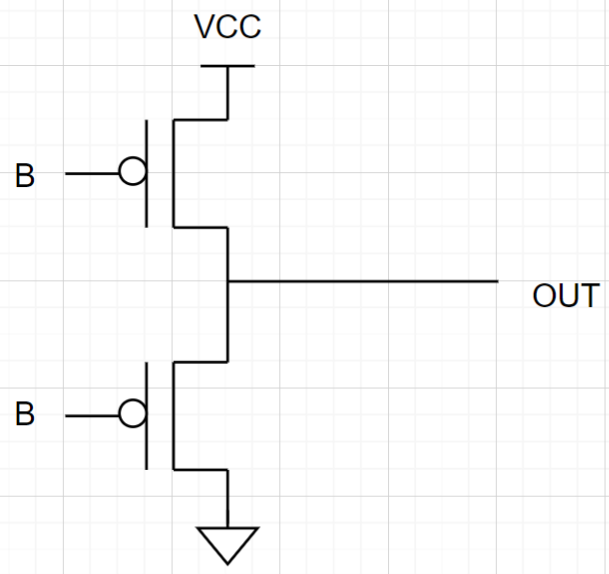
\includegraphics[width=0.6\textwidth]{figures/CMOS_2a.png}
\end{figure}
\newpage

b.
\begin{figure}[!h]
        \centering
        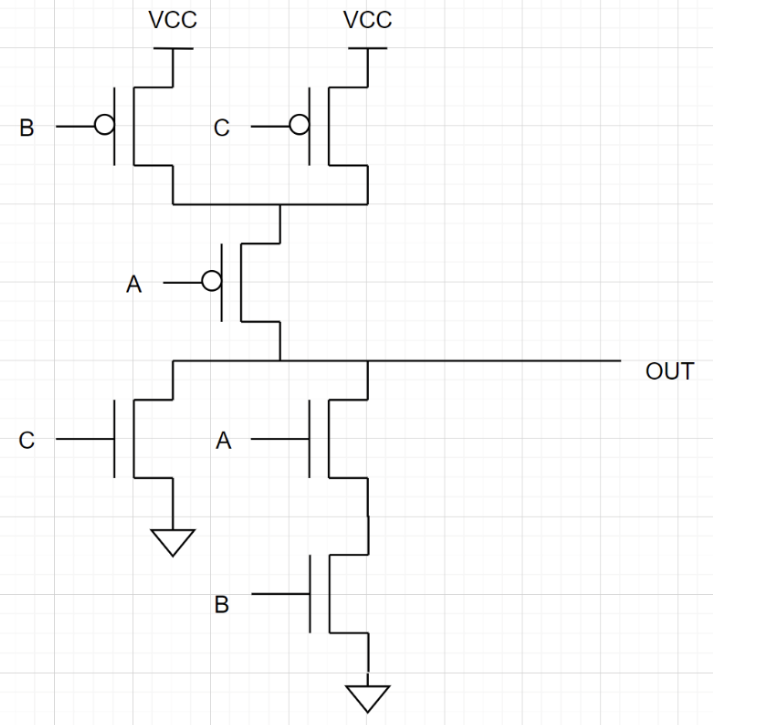
\includegraphics[width=0.9\textwidth]{figures/CMOS_2b.png}
\end{figure}

\newpage
\section*{Boolean Expressions, Algebra, \& Optimization}
\subsection*{Problem 1}
Simplify the following expressions:
\begin{enumerate}[label=\alph*.]
    \item $ F(A,B,C) = (A + B) \cdot (B' + C) \cdot (A + C)$
    \item $ F(A,B,C) = A'BC + ABC + ABC' + AB'C$
    \item $ F(A,B,C) = A' \cdot (A + B) + (A + B) \cdot (A + B')$
\end{enumerate}

\subsection*{Problem 2}
True or False:
\begin{enumerate}[label=\alph*.]
    \item The delay for the following expression is 2.

    \begin{figure}[!h]
        \centering
        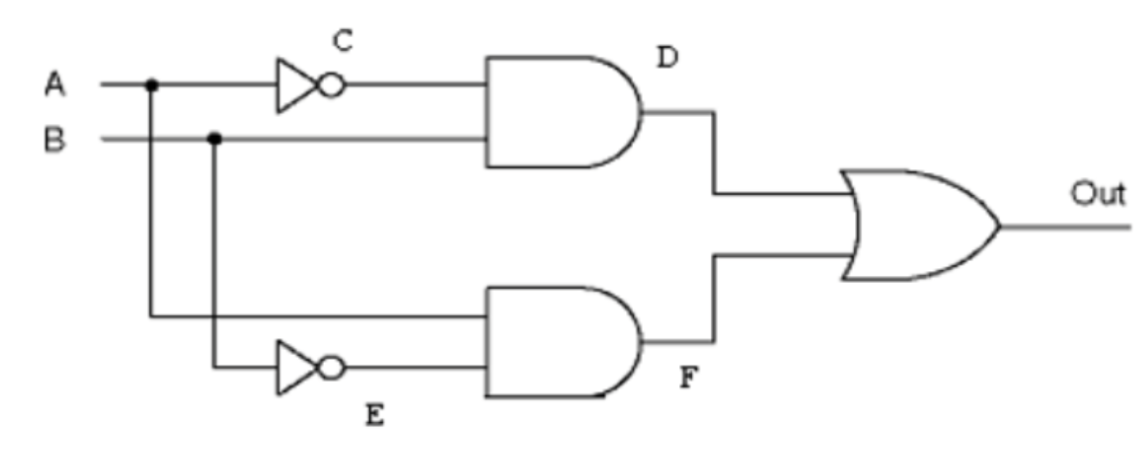
\includegraphics[width=0.7\textwidth]{figures/boolean2a.png}
    \end{figure}
    
    \item The area for the following expression is 7.

    \begin{figure}[!h]
        \centering
        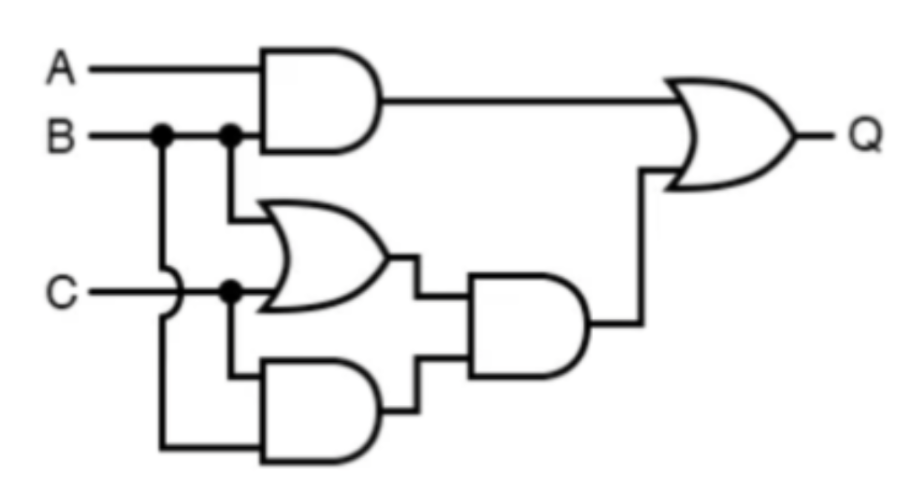
\includegraphics[width=0.7\textwidth]{figures/boolean2b.png}
    \end{figure}
    
\end{enumerate}

\newpage
\section*{K-maps, SOP \& POS Expressions}
\subsection*{Problem 1}
Use K-maps or simplification to find the minimal SOP and POS expressions for the following, then draw them in NAND/NOR form:\\

a. 
    \begin{table}[!h]
    \centering
\begin{tabular}{|c|c|c|c|}
\hline
\textbf{B} & \textbf{C} & \textbf{D} & \textbf{Z} \\ \hline 
0          & 0          & 0          & 1          \\ \hline 
0          & 0          & 1          & 0          \\ \hline 
0          & 1          & 0          & 1          \\ \hline 
0          & 1          & 1          & 1          \\ \hline 
1          & 0          & 0          & 0          \\ \hline 
1          & 0          & 1          & 0          \\ \hline 
1          & 1          & 0          & X          \\ \hline 
1          & 1          & 1          & 1          \\ \hline
\end{tabular}
\end{table} \\
    
b.
\begin{table}[!h]
\centering
\begin{tabular}{|l|l|l|l|l|}
\hline
\textbf{A} & \textbf{B} & \textbf{C} & \textbf{D} & \textbf{Z} \\ \hline
0          & 0          & 0          & 0          & 0          \\ \hline
0          & 0          & 0          & 1          & 1          \\ \hline
0          & 0          & 1          & 0          & 1          \\ \hline
0          & 0          & 1          & 1          & 1          \\ \hline
0          & 1          & 0          & 0          & 0          \\ \hline
0          & 1          & 0          & 1          & 0          \\ \hline
0          & 1          & 1          & 0          & X          \\ \hline
0          & 1          & 1          & 1          & X          \\ \hline
1          & 0          & 0          & 0          & 0          \\ \hline
1          & 0          & 0          & 1          & 1          \\ \hline
1          & 0          & 1          & 0          & 0          \\ \hline
1          & 0          & 1          & 1          & 0          \\ \hline
1          & 1          & 0          & 0          & 0          \\ \hline
1          & 1          & 0          & 1          & X          \\ \hline
1          & 1          & 1          & 0          & X          \\ \hline
1          & 1          & 1          & 1          & X          \\ \hline
\end{tabular}
\end{table}

\newpage
\section*{Adders, ALUs, and Bit-Slicing}
\subsection*{Problem 1}
Remember that the logical output for one slice of a full adder is:
\begin{table}[!h]
\centering
\begin{tabular}{|l|l|l|l|l|}
\hline
\textbf{A} & \textbf{B} & \textbf{Cin} & \textbf{Cout} & \textbf{S} \\ \hline
0          & 0          & 0            & 0             & 0          \\ \hline
0          & 0          & 1            & 0             & 1          \\ \hline
0          & 1          & 0            & 0             & 1          \\ \hline
0          & 1          & 1            & 1             & 0          \\ \hline
1          & 0          & 0            & 0             & 1          \\ \hline
1          & 0          & 1            & 1             & 0          \\ \hline
1          & 1          & 0            & 1             & 0          \\ \hline
1          & 1          & 1            & 1             & 1          \\ \hline
\end{tabular}
\end{table}

\begin{enumerate}[label=\alph*.]
    \item Find an expression for Cout and S using AND and OR gates.
    \item Consider the digital circuit: 
    \begin{figure}[!h]
        \centering
        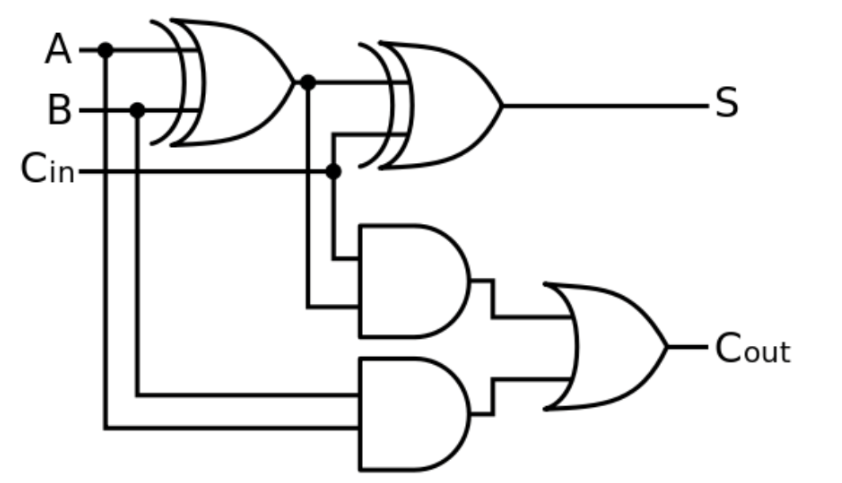
\includegraphics[width=0.7\textwidth]{figures/adder1b.png}
    \end{figure}
    \\ Verify that it is equivalent to your expression.
\end{enumerate}

\subsection*{Problem 2}
Build each of these circuits using only adders, inverters, and fixed inputs (1 or 0). Do not account for overflows unless otherwise noted.
\begin{enumerate}[label=\alph*.]
    \item For two 4-bit unsigned integers $A_3A_2A_1A_0$ and $B_3B_2B_1B_0$, calculate the 5-bit unsigned integer $S_4S_3S_2S_1S_0 = A + B$. 
    \item For two 4-bit two's complement integers $A_3A_2A_1A_0$ and $B_3B_2B_1B_0$ , calculate the 4-bit two's complement integer $S_3S_2S_1A_0$ where $S=A-B$.
    \item For three 3-bit two's complement integers $A_2A_1A_0$, $B_2B_1B_0$, $C_2C_1C_0$, calculate $S_2S_1S_0=A+A-B-C$.
\end{enumerate}


\subsection*{Problem 3}
Assume an ALU that takes two 8-bit integers $A$ and $B$ as input and can calculate $AB$ (AND), 
\begin{enumerate}[label=\alph*.]
    \item How many bits is the output $S$?
    \item How many bits must the control signal be? 
    \item Is the ALU logically complete? Assume you have 0 and 1 available.
    \item (Optional) Draw out the full circuit diagram for this ALU, using basic logic gates, MUXs, decoders, and full adders.
\end{enumerate}


\subsection*{Problem 4}
In 50 or fewer words, explain the advantages and disadvantages of bit-slicing over optimizing for many variables.

\newpage
\section*{Multiplexers}
\subsection*{Problem 1}
Write down the truth table for a 2-to-1 multiplexer. Write an expression for the output, and implement the 2:1 MUX using AND gates, OR gates, and inverters.


\subsection*{Problem 2}
Using the same process (you may not need the truth table), implement a 4:1 MUX using AND gates, OR gates, and inverters.


\subsection*{Problem 3}
Implement a 4:1 MUX using three 2:1 MUXs.


\subsection*{Problem 4}
Implement a 8:1 MUX using two 4:1 MUXs and a 2:1 MUX.
\\ \\
\section*{Decoders}
\subsection*{Problem 1}
In 20 words or less, what does a decoder do?

\subsection*{Problem 2}
Implement a 2x4 decoder using AND gates, OR gates, and inverters.

\subsection*{Problem 3}
Implement a 4x16 decoder using five 2x4 decoders. (Hint: you should use the ENABLE pin)

\newpage
\section*{Latches \& Flip-Flops}
\subsection*{Problem 1}
Find the stable states of the following latches: \\

a.
    \begin{figure}[!h]
        \centering
        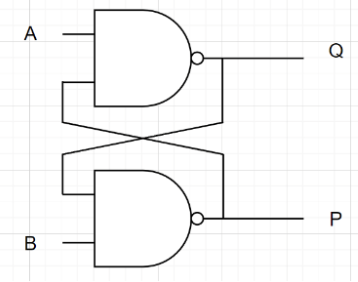
\includegraphics[width=0.7\textwidth]{figures/latch1a.png}
    \end{figure}

b.
    \begin{figure}[!h]
        \centering
        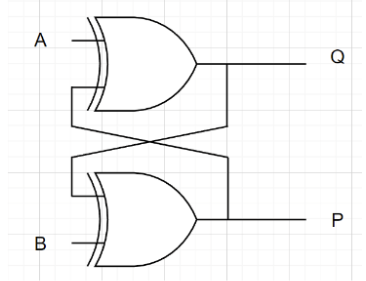
\includegraphics[width=0.7\textwidth]{figures/latch1b.png}
    \end{figure}

c. Which latch is more viable for data storage?

\subsection*{Problem 2}
Explain the process of storing a bit of data in a D latch.
\begin{figure}[!h]
    \centering
    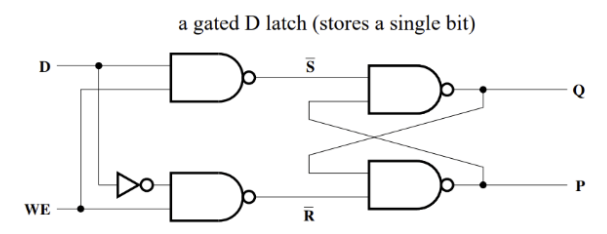
\includegraphics[width=0.7\textwidth]{figures/latch2.png}
\end{figure}


\subsection*{Problem 3}
Explain the difference between a D latch and a D flip-flop.


\subsection*{Problem 4}
Implement a 4-bit register using D flip-flops.


\subsection*{Problem 5}
Implement a 4-bit shift register with MSB load using D flip-flops.


\subsection*{Problem 6}
Implement a 4-bit circular shift register with 4-bit load using D flip-flops.

\newpage
\subsection*{Problem 7}
Consider this digital circuit below. \\
\begin{figure}[!h]
    \centering
    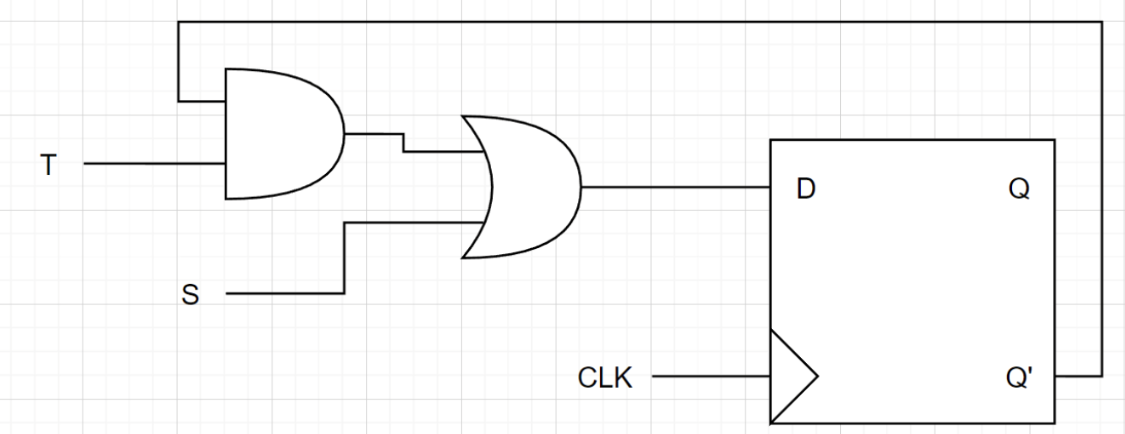
\includegraphics[width=0.7\textwidth]{figures/latch7.png}
\end{figure} \\
Assume at the start, $Q = 0$. Trace and fill out the table below. $T$ and $S$ signals are given in the table.
\begin{table}[!h]
\centering
\begin{tabular}{|l|l|l|l|l|}
\hline
\textbf{Clock Cycle \#} & \textbf{Q} & \textbf{T} & \textbf{S} & \textbf{Qnext} \\ \hline
0                       & 0          & 1          & 0          &                \\ \hline
1                       &            & 1          & 0          &                \\ \hline
2                       &            & 0          & 0          &                \\ \hline
3                       &            & 0          & 0          &                \\ \hline
4                       &            & 0          & 1          &                \\ \hline
\end{tabular}
\end{table}

\subsection*{Problem 8}
What are timing hazards? What are a few ways we can design around them? (Lumetta 2.6.3-2.6.5)

\newpage
\section*{Serialized Design}
\subsection*{Problem 1}
Consider one bit-slice of a full adder.
\begin{enumerate}[label=\alph*.]
    \item How many bits need to be passed between each bit slice? What are they?
    \item If we wanted to serialize this design and add 1 bit at a time, how many D flip-flops would we need to store these signals?
    \item Implement a serialized binary adder, adding 1 bit at a time.
    \item Assume we instead wanted to add 4 bits (1 hexadecimal) at a time. Would any signals be different?
    \item Implement a serialized binary adder, adding 4 bits at a time.
\end{enumerate}


\subsection*{Problem 2}
Consider a serialized circuit that takes a sequence of bits, 1 bit at a time, and outputs the same sequence of bits but is delayed by 2 bits and inverted. For example, assuming inputs and outputs are taken at the start of each clock cycle, if the input is 100101101100, then the output is XX0110100100.
\begin{enumerate}[label=\alph*.]
    \item How many bits do we need to store between each clock cycle?
    \item Implement this circuit using D flip-flops.
    \item Can we also implement this circuit using a shift register?
\end{enumerate}


\subsection*{Problem 3}
In 50 words or less, what are the advantages and disadvantages of serialization over bit-slicing?


\end{document}